\documentclass[aspectratio=169, 10pt]{beamer}

\usetheme{Madrid}
\usecolortheme{default}
\setbeamertemplate{navigation symbols}{}
\setbeamertemplate{footline}[frame number]

\usepackage{booktabs}
\usepackage{graphicx}
\usepackage{amsmath}
\usepackage{xcolor}
\usepackage{tikz}

\definecolor{ctwblue}{RGB}{21,101,192}
\definecolor{ngramred}{RGB}{230,81,0}
\definecolor{gpt2green}{RGB}{46,125,50}
\definecolor{shannonred}{RGB}{183,28,28}

% -----------------------------------------------------------------------
\title[Long-Range Dependency Gap]{Long-Range Dependency Gap in\\
  Character-Level Language Models}
\subtitle{CTW vs.\ N-gram vs.\ GPT-2}
\date{July 22, 2026}
% -----------------------------------------------------------------------

\begin{document}

% ---- Title ----
\begin{frame}
  \titlepage
\end{frame}

% ------------------------------------------------------------------ %
\begin{frame}{Research Question}

  \begin{block}{Motivation}
    Frans Willems' ISIT 2026 Shannon Lecture asked:\\
    \textit{``How much can classical finite-memory models explain about
    natural language — and how far are they from neural LMs?''}
  \end{block}

  \bigskip
  \textbf{Goal:} Quantify the \emph{long-range dependency gap} between:
  \begin{itemize}
    \item \textcolor{ctwblue}{\textbf{CTW}} (Context Tree Weighting) — optimal
          finite-memory coding up to depth $D$
    \item \textcolor{ngramred}{\textbf{N-gram KT}} — same KT estimator, flat backoff
    \item \textcolor{gpt2green}{\textbf{GPT-2}} (small \& large) — Transformer,
          effective context $\approx$ 5000 chars
  \end{itemize}

  \bigskip
  \textbf{Metric:} Bits per character (BPC) $\downarrow$ — lower is better
\end{frame}

% ------------------------------------------------------------------ %
\begin{frame}{Experimental Setup}

  \begin{columns}
    \begin{column}{0.48\textwidth}
      \textbf{Dataset: WikiText-2}
      \begin{itemize}
        \item Normalized to 28-char alphabet\\
              $\{$\texttt{a--z}, space, newline$\}$
        \item Train: \textbf{10\,M chars}
        \item Validation: \textbf{1\,M chars}
      \end{itemize}

      \bigskip
      \textbf{Models}
      \begin{itemize}
        \item CTW depths $D \in \{3, 5, 7, 10\}$
        \item N-gram KT orders $\in \{4, 6, 8, 11\}$
        \item GPT-2 small (117\,M params)
        \item GPT-2 large (774\,M params)
      \end{itemize}
    \end{column}
    \begin{column}{0.48\textwidth}
      \textbf{CTW key parameters}
      \begin{itemize}
        \item KT estimator at every node:\\
              $P_e(s) = \dfrac{n_s + \tfrac{1}{2}}{n + \tfrac{A}{2}}$
        \item Mixing weight $\alpha = 0.5$ (training)
        \item Prediction weight $\alpha_p = 0.1$ (evaluation)
        \item Backoff threshold $n_{\min} = 15$
      \end{itemize}

      \bigskip
      \textbf{Second dataset}
      \begin{itemize}
        \item text8 (enwiki) — replicated all experiments
      \end{itemize}
    \end{column}
  \end{columns}
\end{frame}

% ------------------------------------------------------------------ %
\begin{frame}{Main Results: BPC vs.\ Context Depth}

  \begin{center}
    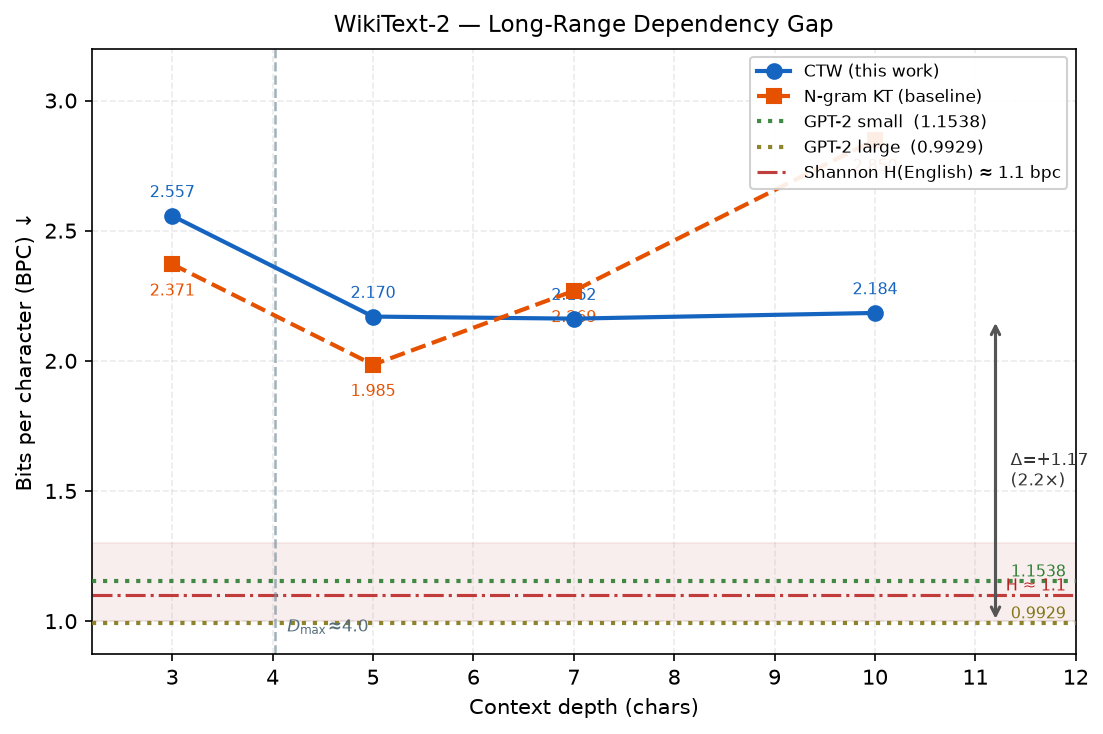
\includegraphics[width=0.75\textwidth]{experiments/bpc_plot.png}
  \end{center}

  \vspace{-4pt}
  \small
  \begin{tabular}{lrr}
    \toprule
    Model & BPC $\downarrow$ & vs.\ CTW best \\
    \midrule
    N-gram 6-gram (best) & 1.985 & $-0.18$  \\
    \textcolor{ctwblue}{CTW $D=7$ (best)} & \textcolor{ctwblue}{\textbf{2.162}} & — \\
    \textcolor{gpt2green}{GPT-2 small} & \textcolor{gpt2green}{1.154} & $-1.01$ \\
    \textcolor{gpt2green}{GPT-2 large} & \textcolor{gpt2green}{0.993} & $-1.17$ \\
    \textcolor{shannonred}{Shannon $H$(English)} & \textcolor{shannonred}{$\approx 1.1$} & \\
    \bottomrule
  \end{tabular}
\end{frame}

% ------------------------------------------------------------------ %
\begin{frame}{Surprising Finding: N-gram Beats CTW}

  \begin{columns}
    \begin{column}{0.52\textwidth}
      \centering
      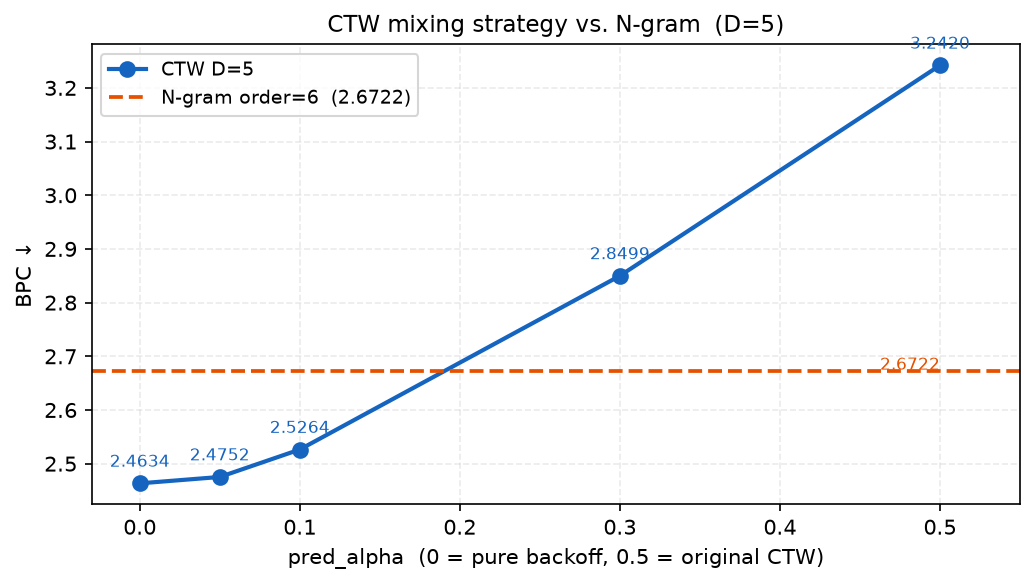
\includegraphics[width=\textwidth]{experiments/ctw_backoff_results.png}
    \end{column}
    \begin{column}{0.45\textwidth}
      \textbf{Why does N-gram outperform CTW?}

      \smallskip
      CTW blends predictions from \emph{all} tree levels:
      \[
        P_{\text{pred}} = (1-\alpha_p)\,P_{\text{leaf}} + \alpha_p\,P_{\text{parent}}
      \]
      For depth $D=5$ with $\alpha_p=0.1$:
      \[
        0.9^5 \approx 59\%\ \text{weight on leaf}
      \]
      N-gram uses 100\% of deepest available context.

      \bigskip
      \textbf{Ablation result:}
      \begin{itemize}
        \item $\alpha_p = 0.0$: BPC = 2.463 (best CTW)
        \item $\alpha_p = 0.1$: BPC = 2.526 (default)
        \item $\alpha_p = 0.5$: BPC = 3.242 (original CTW)
        \item N-gram 6-gram: BPC = 2.672 (500K subset)
      \end{itemize}
      $\Rightarrow$ pure backoff ($\alpha_p=0$) is optimal for offline prediction
    \end{column}
  \end{columns}
\end{frame}

% ------------------------------------------------------------------ %
\begin{frame}{Where Is the Gap Largest?}

  \begin{center}
    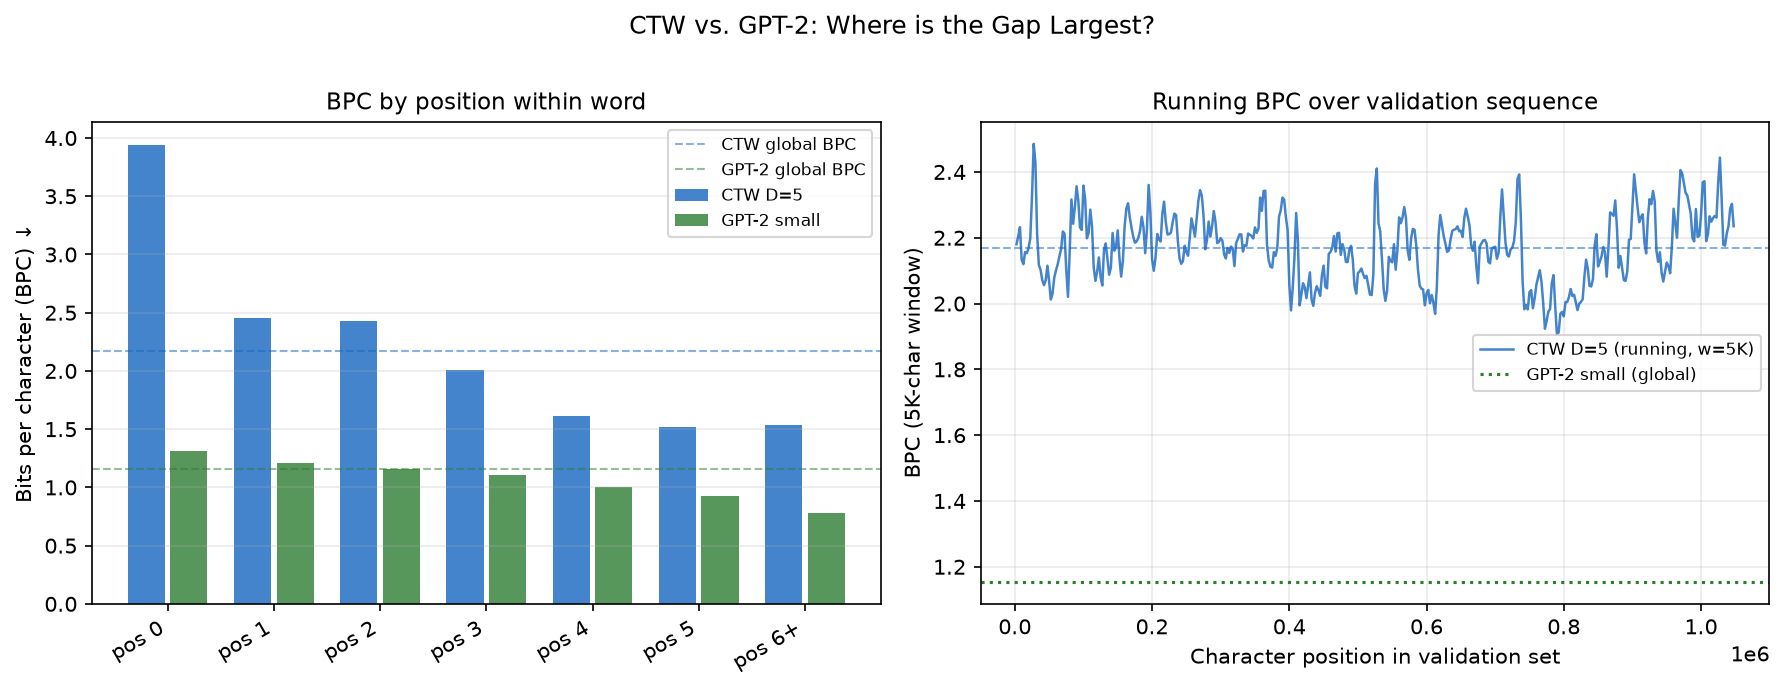
\includegraphics[width=0.80\textwidth]{experiments/gap_analysis_results.png}
  \end{center}

  \vspace{-4pt}
  \begin{columns}
    \begin{column}{0.55\textwidth}
      \small
      \begin{tabular}{lrrr}
        \toprule
        Position & CTW & GPT-2 & Gap \\
        \midrule
        0 — word start & 3.941 & 1.313 & \textbf{+2.63} \\
        1              & 2.456 & 1.207 & +1.25 \\
        2              & 2.428 & 1.155 & +1.27 \\
        5+             & 1.519 & 0.924 & +0.60 \\
        \bottomrule
      \end{tabular}
    \end{column}
    \begin{column}{0.42\textwidth}
      \textbf{Key finding:}\\
      The gap is \emph{4$\times$ larger at word starts}
      than deep within words.

      \smallskip
      Predicting the first letter of the next word
      requires knowing which word will appear —
      a semantic dependency CTW cannot resolve.
    \end{column}
  \end{columns}
\end{frame}

% ------------------------------------------------------------------ %
\begin{frame}{Is the Comparison Fair? Fine-Tuning GPT-2}

  \begin{columns}
    \begin{column}{0.52\textwidth}
      \centering
      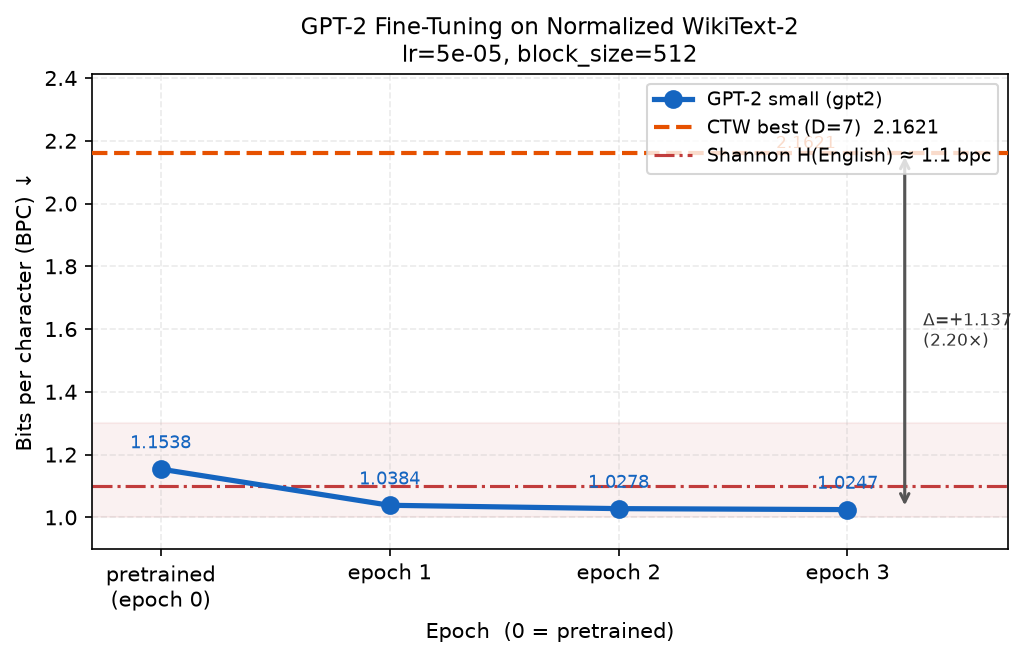
\includegraphics[width=\textwidth]{experiments/finetune_results_20260721_162904.png}
    \end{column}
    \begin{column}{0.45\textwidth}
      \textbf{Concern:} GPT-2 was pretrained on rich text;
      evaluating on 28-char normalized text may inflate the gap.

      \bigskip
      \textbf{Experiment:} Fine-tune GPT-2 small
      on the same 10\,M normalized chars (3 epochs).

      \bigskip
      \begin{tabular}{lr}
        \toprule
        Model & BPC \\
        \midrule
        Pretrained & 1.154 \\
        Fine-tuned ep.\ 1 & 1.038 \\
        Fine-tuned ep.\ 3 & \textbf{1.025} \\
        CTW $D=7$ & 2.162 \\
        \bottomrule
      \end{tabular}

      \bigskip
      $\Rightarrow$ Fine-tuning \emph{widens} the gap to
      $\Delta = 1.14$ bpc ($2.2\times$).\\
      The gap is \textbf{real}, not an artifact.
    \end{column}
  \end{columns}
\end{frame}

% ------------------------------------------------------------------ %
\begin{frame}{Theoretical Saturation Depth $D_{\max}$}

  \begin{columns}
    \begin{column}{0.55\textwidth}
      \centering
      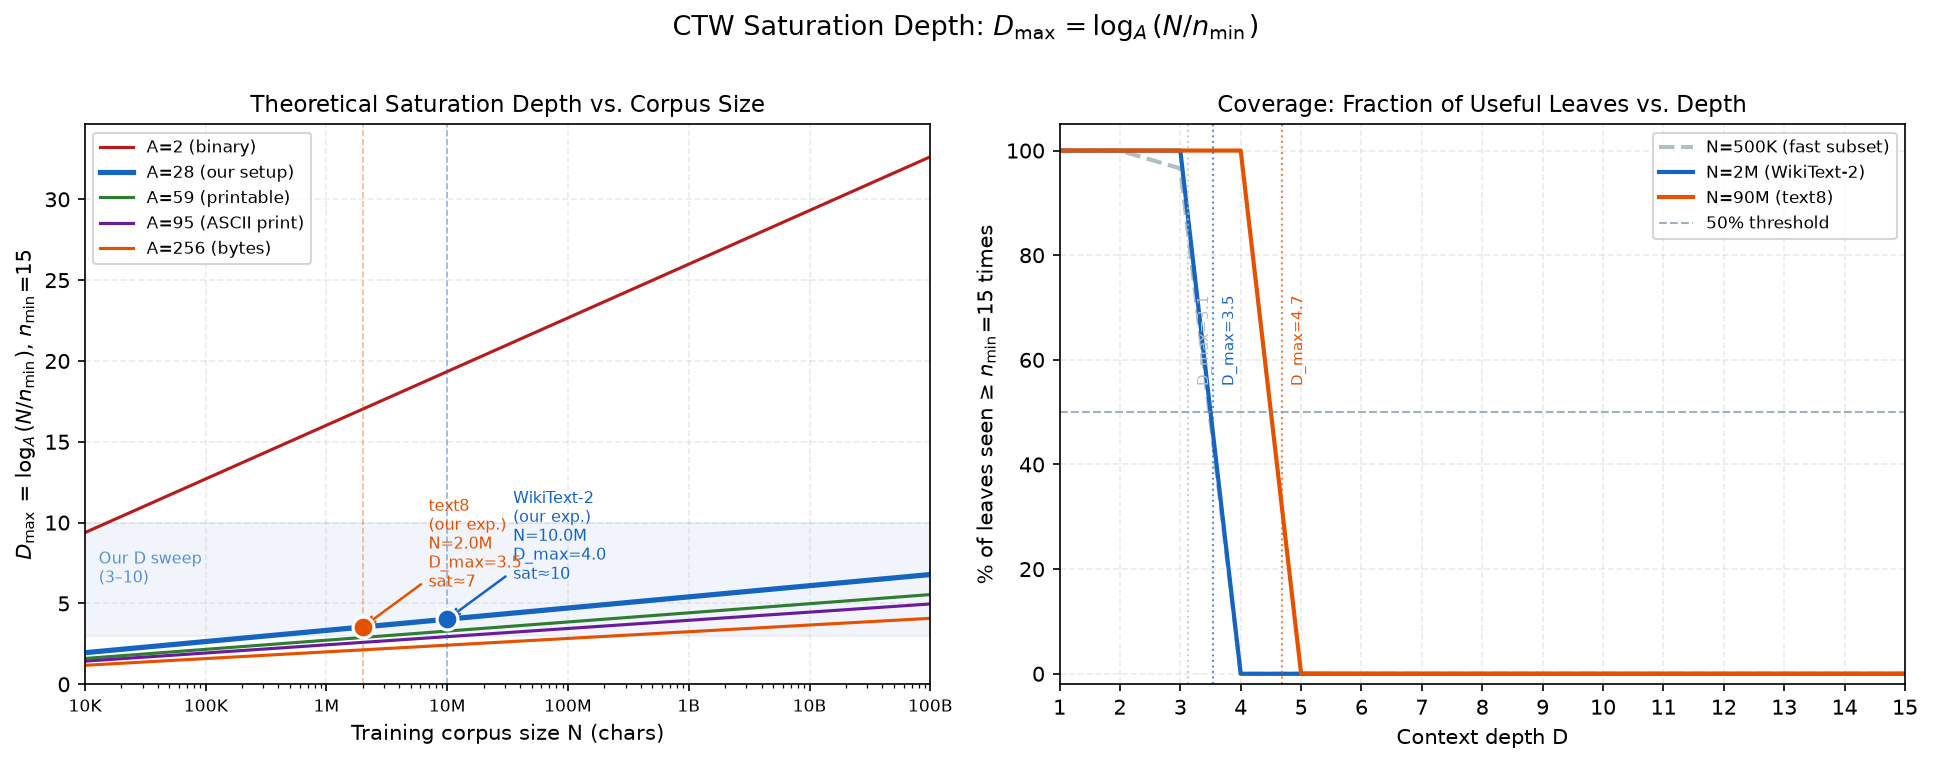
\includegraphics[width=\textwidth]{experiments/dmax_theory.png}
    \end{column}
    \begin{column}{0.42\textwidth}
      \textbf{Formula:}
      \[
        D_{\max} = \log_A\!\left(\frac{N}{n_{\min}}\right)
      \]

      \textbf{Our setup} ($N=10\text{M}$, $A=28$, $n_{\min}=15$):
      \[
        D_{\max} \approx 4.0
      \]

      \bigskip
      \textbf{Implication:}\\
      Beyond $D \approx 4$, most tree leaves have
      $< 15$ training samples — backoff fires everywhere.

      \smallskip
      This explains why BPC at $D=7$ (2.162) and
      $D=10$ (2.184) are nearly identical.

      \bigskip
      \textbf{Theory $\Leftrightarrow$ practice:} empirical
      saturation matches $D_{\max}$.
    \end{column}
  \end{columns}
\end{frame}

% ------------------------------------------------------------------ %
\begin{frame}{Token-level CTW: Word-Granularity Experiments}

  \begin{columns}
    \begin{column}{0.56\textwidth}
      \centering
      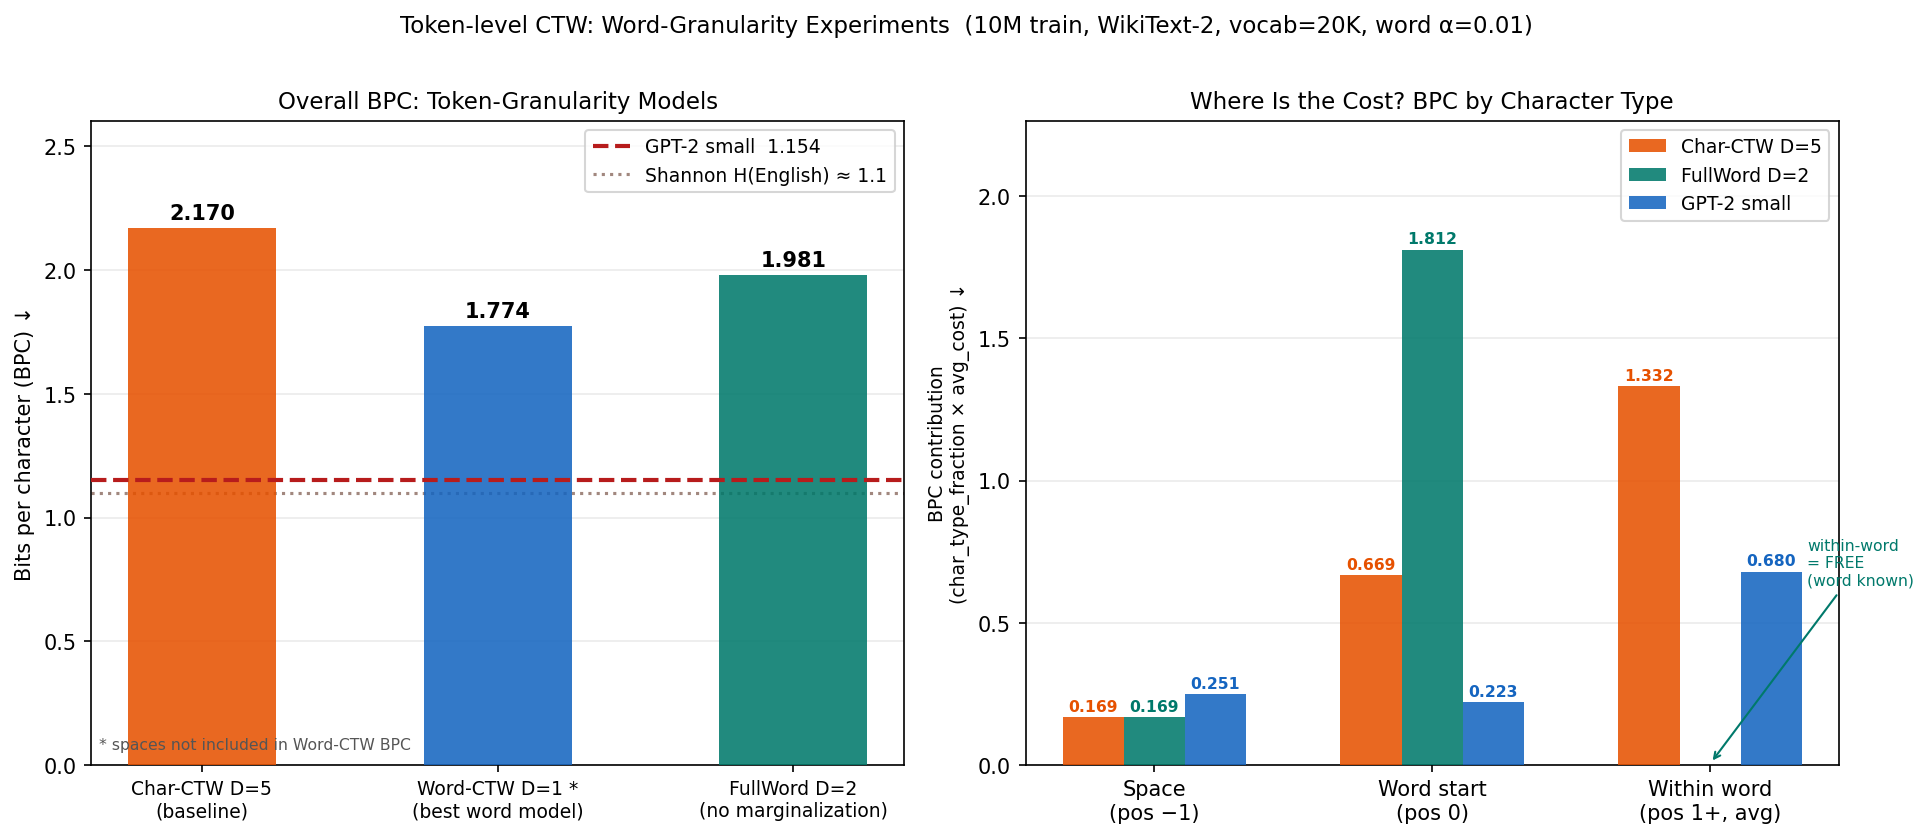
\includegraphics[width=\textwidth]{experiments/token_ctw_plot.png}
    \end{column}
    \begin{column}{0.41\textwidth}
      \textbf{Three variants (10\,M train, vocab=20\,K):}
      \smallskip

      \begin{tabular}{lr}
        \toprule
        Model & BPC \\
        \midrule
        Char-CTW $D=5$ & 2.170 \\
        Word-CTW $D=1$ * & 1.774 \\
        FullWord $D=2$ & \textbf{1.981} \\
        GPT-2 small & 1.154 \\
        \bottomrule
      \end{tabular}
      {\footnotesize * spaces not counted}

      \bigskip
      \textbf{Key findings:}
      \begin{itemize}
        \item \textbf{Within-word chars are free} in FullWord\\
              (word identity determines all of them)
        \item Word-start cost dominates: \textbf{1.81} bpc\\
              vs.\ 0.67 for Char-CTW, 0.22 for GPT-2
        \item $D_{\max} \approx 1.3$ confirmed: $D=2$ worse\\
              than $D=1$ for word-level model
        \item Gap to GPT-2 shrinks to $\Delta \approx 0.83$\\
              but fundamental barrier remains
      \end{itemize}
    \end{column}
  \end{columns}
\end{frame}

% ------------------------------------------------------------------ %
\begin{frame}{$\mathrm{BPC}_{\min}(D)$: Lower Bound for Any $D$-Memory Model}

  \begin{center}
    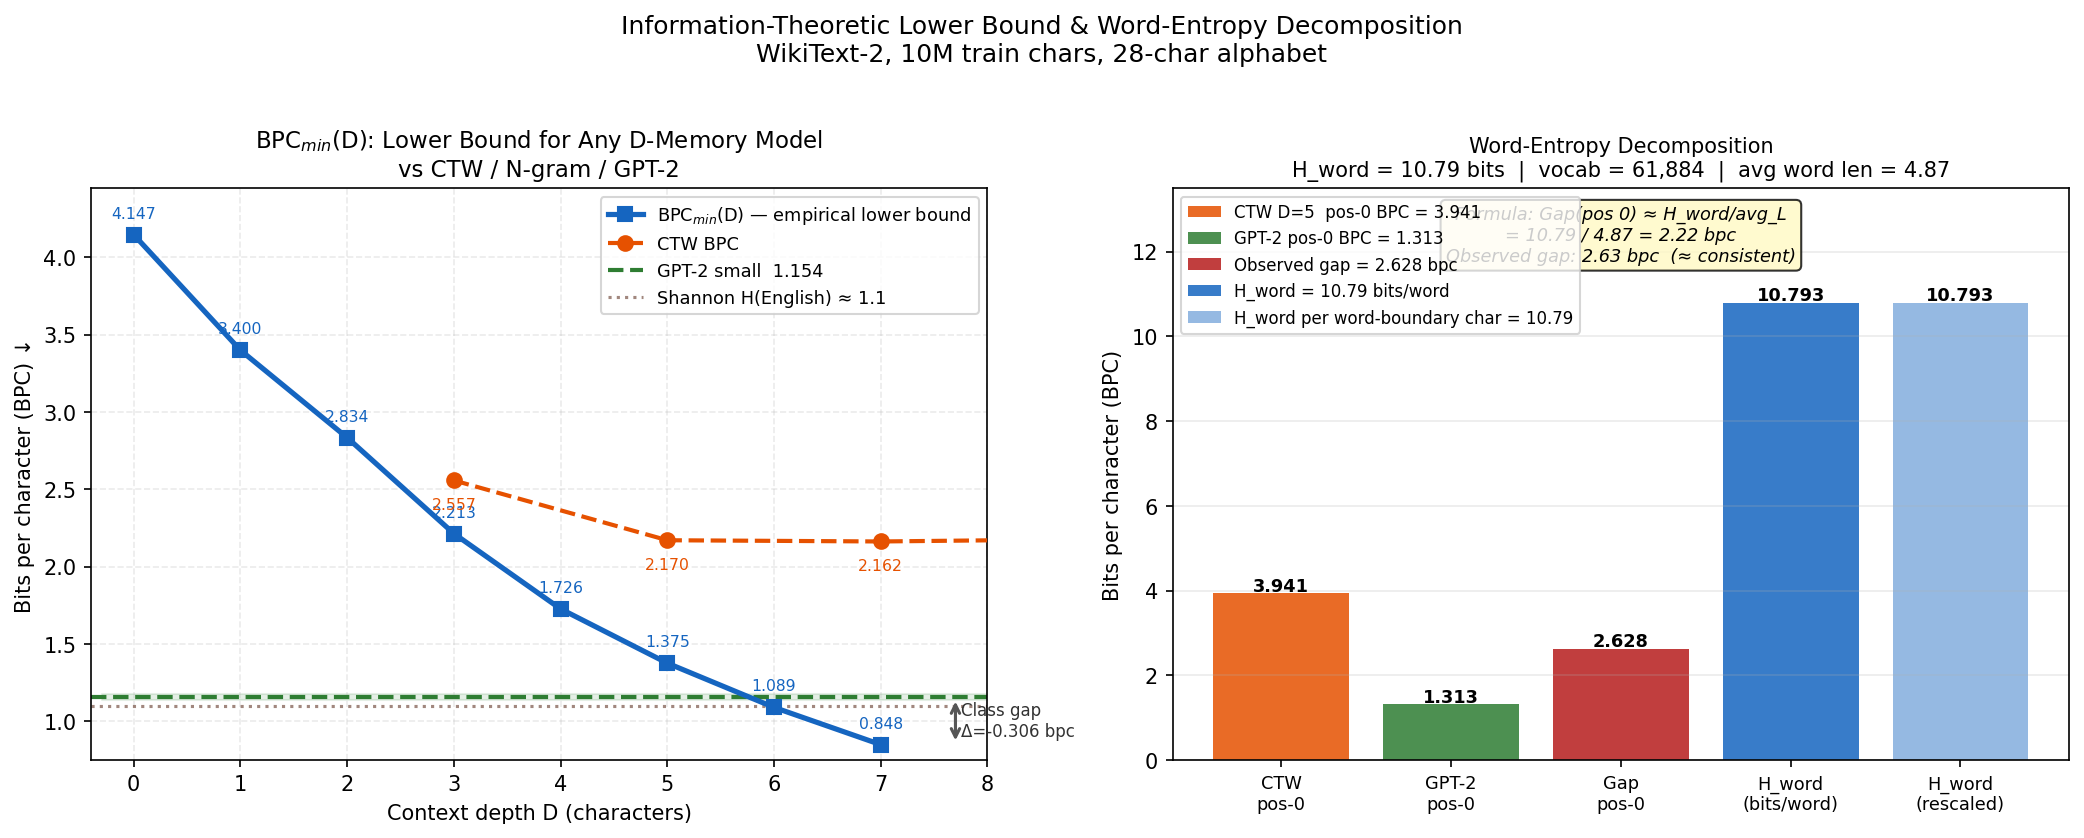
\includegraphics[width=0.76\textwidth]{experiments/bpc_min_plot.png}
  \end{center}

  \vspace{-6pt}
  \small
  \begin{columns}
    \begin{column}{0.55\textwidth}
      \begin{tabular}{lrrr}
        \toprule
        Model & $D$ & BPC & Gap to GPT-2 \\
        \midrule
        $\mathrm{BPC}_{\min}$ & 5 & 1.641 & $+0.49$ \\
        $\mathrm{BPC}_{\min}$ & 7 & \textbf{1.205} & $+0.05$ \\
        CTW & 7 & 2.162 & $+1.01$ \\
        GPT-2 small & — & 1.154 & — \\
        \bottomrule
      \end{tabular}
    \end{column}
    \begin{column}{0.42\textwidth}
      \textbf{Surprising finding:}\\
      $\mathrm{BPC}_{\min}(D{=}7) \approx 1.2$ is near GPT-2 —
      the \emph{class gap} is only $\approx 0.05$ bpc.

      \smallskip
      CTW lags BPC$_{\min}$ by $0.96$ bpc
      due to \textbf{data scarcity} ($D_{\max} \approx 4$).

      \smallskip
      $\Rightarrow$ The CTW–GPT-2 gap is not a
      fundamental class barrier, but a
      \textbf{training-data problem.}
    \end{column}
  \end{columns}
\end{frame}

% ------------------------------------------------------------------ %
\begin{frame}{Conclusions}

  \begin{block}{Main Result}
    \textbf{CTW $D=7$: 2.162 BPC} vs.\
    \textbf{GPT-2 large: 0.993 BPC} $\Rightarrow$
    gap of \textbf{1.17 bits/char} ($\mathbf{2.25\times}$ more uncertainty)
  \end{block}

  \bigskip
  \begin{enumerate}
    \item \textbf{Gap source:} concentrated at word-initial positions\\
          ($+2.63$ bpc at pos 0 vs.\ $+0.60$ bpc at pos 5+)\\
          $\Rightarrow$ CTW lacks semantic/syntactic long-range context

    \item \textbf{Mixing vs.\ backoff:} pure backoff ($\alpha_p=0$) is optimal for
          offline prediction; original CTW mixing hurts by $+0.78$ bpc

    \item \textbf{Fair comparison:} fine-tuning GPT-2 on same data
          widens the gap ($1.154 \to 1.025$ BPC), not narrows it

    \item \textbf{Saturation:} $D_{\max} \approx 4$ explains why
          going beyond $D=5$ yields no improvement

    \item \textbf{Lower bound:} $\mathrm{BPC}_{\min}(D{=}7) \approx 1.20$
          is only $0.05$ bpc above GPT-2 — the class gap is negligible;
          the CTW–GPT-2 gap is a \emph{data-scarcity} barrier

    \item \textbf{Broader context:} GPT-2 large ($\approx 0.99$ bpc)
          approaches Shannon entropy ($\approx 1.1$ bpc) —
          neural LMs have essentially ``solved'' character-level English
  \end{enumerate}
\end{frame}

% ------------------------------------------------------------------ %
\begin{frame}{Future Directions \hfill \small\textcolor{gray}{toward a paper}}

  \begin{columns}[T]
    \begin{column}{0.47\textwidth}

      \textbf{\textcolor{ctwblue}{Empirical}}
      \smallskip

      \begin{enumerate}
        \item \textbf{PPM/PPMD baseline}\\
              Classical compression SOTA ($\approx$2.0 bpc).\\
              Completes the picture:\\
              CTW $\to$ N-gram $\to$ PPM $\to$ GPT-2.

        \item \textbf{Mutual information curve}\\
              $I(X_t;\, X_{t-d})$ vs.\ lag $d$ —\\
              shows how much long-range information
              exists in the corpus at each distance.

        \item \textbf{Small LSTM baseline}\\
              Fills the space between CTW and GPT-2;
              shows even a tiny neural model captures
              what CTW cannot.
      \end{enumerate}

    \end{column}
    \begin{column}{0.50\textwidth}

      \textbf{\textcolor{gpt2green}{Theoretical}}
      \smallskip

      \begin{enumerate}
        \setcounter{enumi}{3}
        \item \textbf{Information-theoretic lower bound \checkmark}\\[2pt]
              $\mathrm{BPC}_{\min}(D) = H(X_t \mid X_{t-D{:}t-1})$
              computed — see previous slide.\\[3pt]
              \textbf{Revised claim:} gap is a \emph{data-scarcity}
              barrier, not a class barrier
              ($\mathrm{BPC}_{\min}(7) \approx$ GPT-2).

        \item \textbf{Word-entropy decomposition}\\[2pt]
              $\text{Gap} \approx H_{\text{word}}\,/\,\bar{L}$
              at word boundaries,\\
              where $H_{\text{word}}$ = word unigram entropy,
              $\bar{L}$ = avg.\ word length.\\
              Turns an observation into a \emph{formula}.
      \end{enumerate}

    \end{column}
  \end{columns}
\end{frame}

% ------------------------------------------------------------------ %
\begin{frame}{Backup: Two-Dataset Validation}
  \begin{center}
    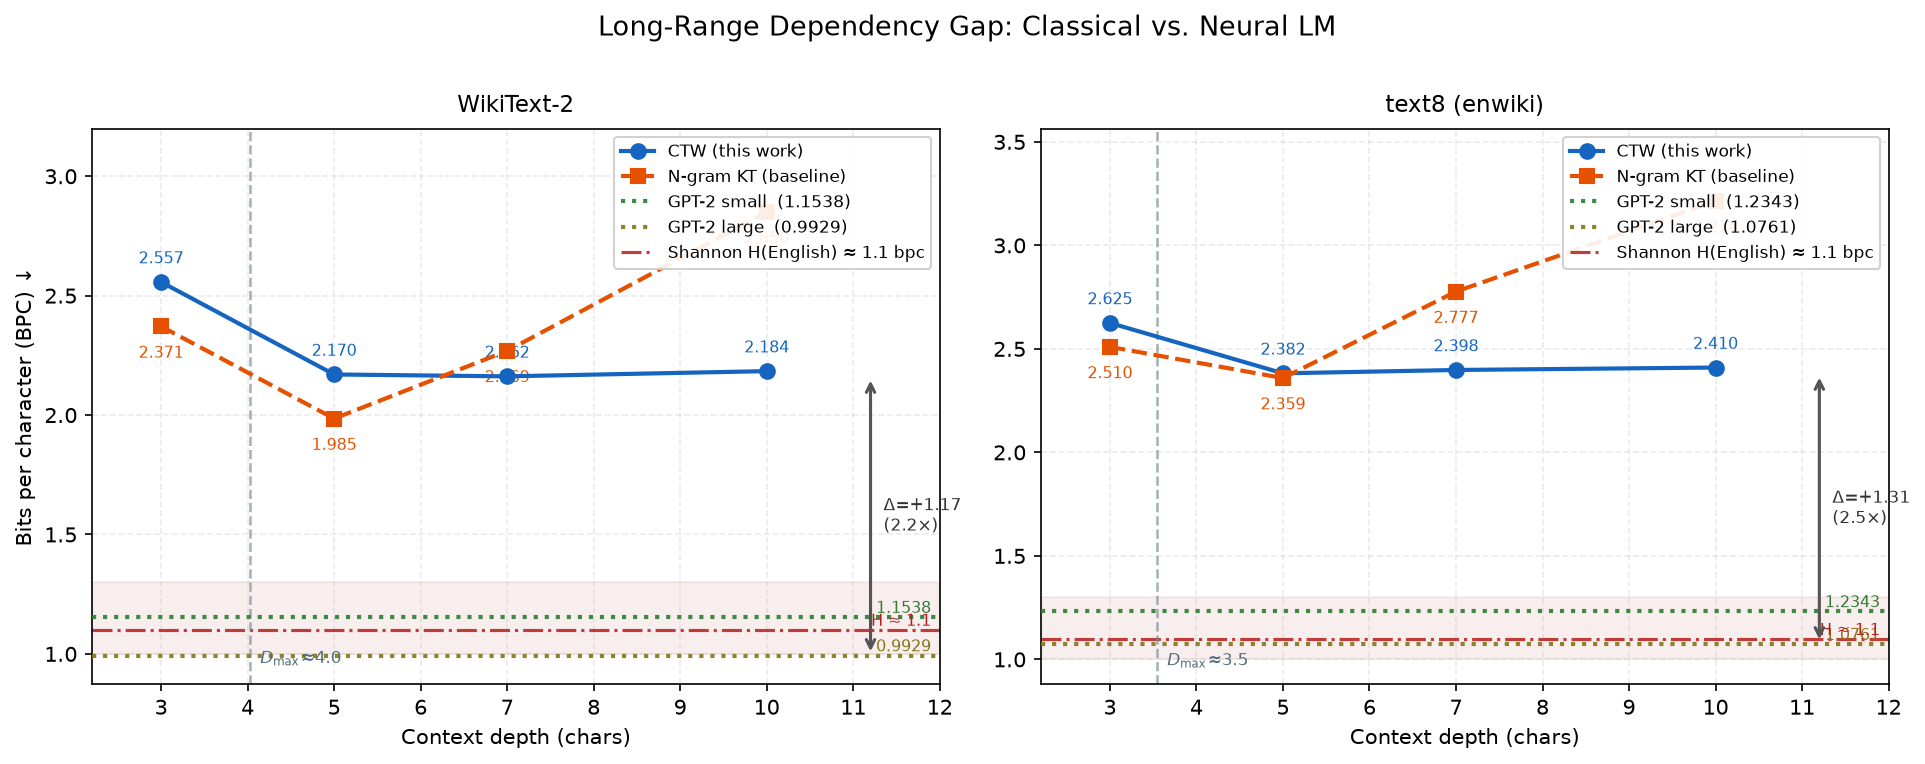
\includegraphics[width=0.88\textwidth]{experiments/bpc_plot_2panel.png}
  \end{center}
  \vspace{-4pt}
  \small
  Gap is consistent across WikiText-2 and text8 (enwiki) — result is dataset-agnostic.
\end{frame}

\end{document}
